% !TeX program = xelatex
% !TeX root = retrieval_project_report.tex
\documentclass[11pt,a4paper]{article}

\usepackage[margin=1.8cm]{geometry}
\usepackage{microtype}
\usepackage{amsmath,amssymb}
\usepackage{booktabs}
\usepackage{longtable}
\usepackage{array}
\usepackage{hyperref}
\usepackage{listings}
\usepackage{tikz}

\usetikzlibrary{arrows.meta, positioning, shapes.geometric, calc}

\hypersetup{
  colorlinks=true,
  linkcolor=blue!50!black,
  urlcolor=teal!50!black,
  pdftitle={Retrieval Engine Competition Project},
  pdfauthor={Maksym DOLHOV; Mehdi AGHAEI; Nguyen Ho Bao KHANH},
  pdfsubject={SeaFour project report},
  pdfcreator={},
  pdfproducer={}
}

\setlength{\parindent}{0pt}
\setlength{\parskip}{6pt}
\renewcommand{\arraystretch}{1.2}

\definecolor{ink}{HTML}{213547}
\definecolor{softblue}{HTML}{DCEAF7}
\definecolor{softgreen}{HTML}{DFF4E5}
\definecolor{softorange}{HTML}{F8EAD7}
\definecolor{softrose}{HTML}{F7DBE6}
\definecolor{softgold}{HTML}{F8F2CF}

\lstdefinestyle{codeblock}{
  basicstyle=\ttfamily\small,
  breaklines=true,
  columns=fullflexible,
  keepspaces=true,
  frame=single,
  framesep=4pt,
  rulecolor=\color{ink!30},
  backgroundcolor=\color{softblue!25}
}
\lstset{style=codeblock}

\newcommand{\studybox}[2]{%
  \par\medskip
  \noindent\fcolorbox{ink}{white}{%
    \parbox{0.96\linewidth}{\textbf{#1}\par #2}%
  }%
  \par\medskip
}

\begin{document}

% ─────────────────────────── Title page ──────────────────────────────────────
\begin{titlepage}
\centering
{\Large \textbf{Retrieval Engine Competition Project}}\\[0.6cm]
{\large Project Report}\\[0.6cm]
{\large Group: SeaFour}\\[0.8cm]

\begin{tabular}{c}
Maksym DOLHOV \\
Mehdi AGHAEI \\
Nguyen Ho Bao KHANH \\
\end{tabular}\\[1.2cm]

\studybox{Project Scope}{%
This report documents the notebook-based submission workflow for the Kaggle
retrieval competition. The implementation lives in
\texttt{kaggle/kaggle\_submission.ipynb}, which loads the competition data,
preprocesses text, runs four retrieval methods (TF-IDF, BM25+, Embedding
Search, and a Hybrid BM25+\,+\,Embedding re-ranking approach), evaluates
them on the training set, and writes the final submission CSV with the best
model.}

\vspace{0.6cm}

\begin{tabular}{>{\bfseries}p{0.28\linewidth} p{0.58\linewidth}}
Main workflow   & \texttt{kaggle/kaggle\_submission.ipynb} \\
Submission file & \texttt{kaggle/solutions\_SeaFour.csv} \\
Report          & \texttt{reports/retrieval\_project\_report.pdf} \\
Date            & \today \\
\end{tabular}

\vfill
\end{titlepage}

% ═══════════════════════════════════════════════════════════════════════════════
\section{Project At A Glance}
% ═══════════════════════════════════════════════════════════════════════════════

The submission workflow is notebook-first.
One Kaggle notebook contains all the logic needed to reproduce the submission file:

\begin{itemize}
\item \texttt{kaggle/kaggle\_submission.ipynb} — active implementation.
\item \texttt{kaggle/solutions\_SeaFour.csv} — generated Kaggle-format output.
\item \texttt{reports/retrieval\_project\_report.pdf} — this report.
\end{itemize}

\subsection{Repository Layout}

\begin{tabular}{p{0.29\linewidth} p{0.63\linewidth}}
\toprule
\textbf{Path} & \textbf{Purpose} \\
\midrule
\texttt{data/}             & Competition files: documents, queries, ground-truth, and sample submission. \\
\texttt{kaggle/}        & Active notebook and generated CSV. \\
\texttt{reports/}           & LaTeX source and compiled PDF. \\
\texttt{requirements.txt}  & Python dependencies. \\
\bottomrule
\end{tabular}

\subsection{Pipeline Overview}

\begin{center}
\resizebox{0.98\linewidth}{!}{%
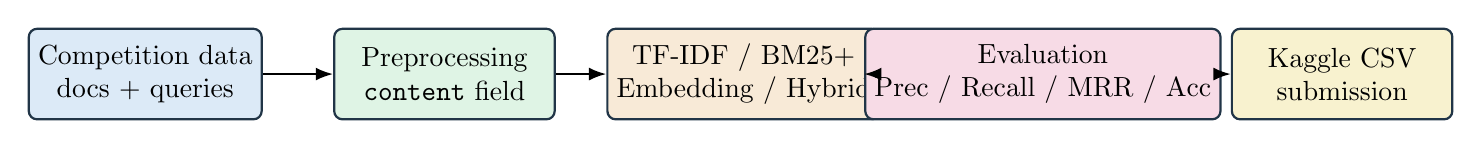
\begin{tikzpicture}[
  box/.style={draw=ink, rectangle, rounded corners=3pt, minimum width=2.8cm,
              minimum height=1.15cm, align=center, thick},
  >={Latex[length=2.2mm]}
]
\node[box, fill=softblue]   (data)   at (0,0)     {Competition data\\docs + queries};
\node[box, fill=softgreen]  (prep)   at (3.8,0)   {Preprocessing\\\texttt{content} field};
\node[box, fill=softorange] (models) at (7.6,0)   {TF-IDF / BM25+\\Embedding / Hybrid};
\node[box, fill=softrose]   (eval)   at (11.4,0)  {Evaluation\\Prec / Recall / MRR / Acc};
\node[box, fill=softgold]   (csv)    at (15.2,0)  {Kaggle CSV\\submission};

\draw[->, thick] (data) -- (prep);
\draw[->, thick] (prep) -- (models);
\draw[->, thick] (models) -- (eval);
\draw[->, thick] (eval) -- (csv);
\end{tikzpicture}
}
\end{center}

% ═══════════════════════════════════════════════════════════════════════════════
\section{Improvement Journey}
% ═══════════════════════════════════════════════════════════════════════════════

We iterated through several submission cycles. The scores below reflect the
latest validated leaderboard results; pending variants are marked as TBD.

\begin{center}
\begin{tabular}{p{0.18\linewidth} p{0.60\linewidth} r}
\toprule
\textbf{Iteration} & \textbf{Main improvement} & \textbf{Score} \\
\midrule
Baseline & Initial lexical pipeline (TF-IDF / BM25+) with shared \texttt{content} field. & 0.16934 \\
Embedding search & Added Sentence-Transformer retrieval for semantic matching. & 0.22592 \\
Hybrid re-ranking & Lexical candidates re-ranked with embeddings + tuned candidate/Top-K. & \textit{TBD} \\
Final system & Refined preprocessing, parameter tuning, and submission pipeline hardening. & \textit{TBD} \\
\bottomrule
\end{tabular}
\end{center}

\studybox{Key Work Items}{%
\begin{itemize}
\item Normalised the text pipeline (lowercasing, separator handling, tag joining).
\item Implemented and compared TF-IDF, BM25+, and embedding-based retrieval.
\item Built the hybrid re-ranking path and tuned \texttt{TOP\_K} and candidate sizes.
\item Hardened the Kaggle submission writer and local/Kaggle path detection.
\end{itemize}}

% ═══════════════════════════════════════════════════════════════════════════════
\section{Dataset}
% ═══════════════════════════════════════════════════════════════════════════════

\begin{tabular}{>{\bfseries}l r l}
\toprule
         & \textbf{Count} & \textbf{File} \\
\midrule
Documents       & 216{,}041 & \texttt{docs.json} \\
Training queries &     327 & \texttt{queries\_train.json} \\
Test queries     &     141 & \texttt{queries\_test.json} \\
Training qrels   &     327 & \texttt{qgts\_train.json} \\
\bottomrule
\end{tabular}

\medskip
Each document has fields \texttt{id}, \texttt{text}, \texttt{title}, \texttt{tags} (list), and \texttt{category}.
The five categories and their document counts:

\begin{center}
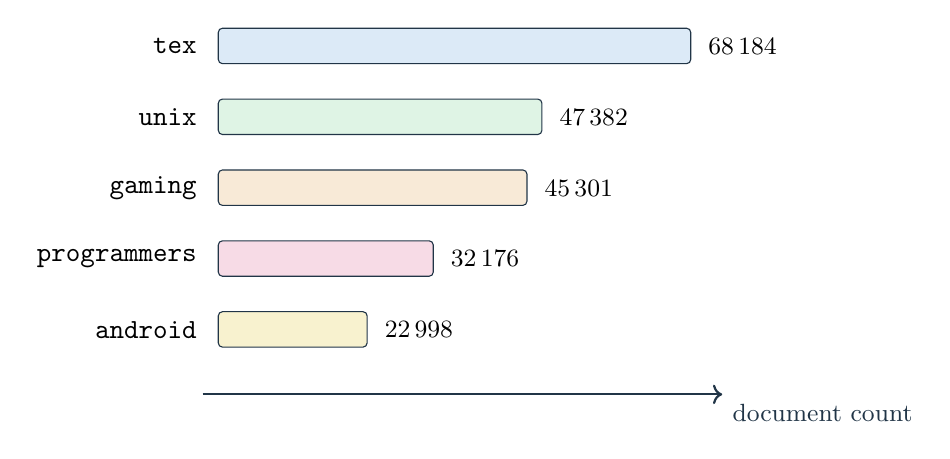
\begin{tikzpicture}[x=1cm,y=1cm]
\draw[->, thick, color=ink] (0,0.6) -- (6.6,0.6) node[below right] {\small document count};
\filldraw[fill=softblue, draw=ink, rounded corners=1.5pt]   (0.2,4.8) rectangle (6.20,5.25);
\node[anchor=east] at (0.05,5.02)  {\texttt{tex}};
\node[anchor=west] at (6.30,5.02)  {\small 68\,184};

\filldraw[fill=softgreen, draw=ink, rounded corners=1.5pt]  (0.2,3.9) rectangle (4.31,4.35);
\node[anchor=east] at (0.05,4.12)  {\texttt{unix}};
\node[anchor=west] at (4.41,4.12)  {\small 47\,382};

\filldraw[fill=softorange, draw=ink, rounded corners=1.5pt] (0.2,3.0) rectangle (4.12,3.45);
\node[anchor=east] at (0.05,3.22)  {\texttt{gaming}};
\node[anchor=west] at (4.22,3.22)  {\small 45\,301};

\filldraw[fill=softrose, draw=ink, rounded corners=1.5pt]   (0.2,2.1) rectangle (2.93,2.55);
\node[anchor=east] at (0.05,2.32)  {\texttt{programmers}};
\node[anchor=west] at (3.03,2.32)  {\small 32\,176};

\filldraw[fill=softgold, draw=ink, rounded corners=1.5pt]   (0.2,1.2) rectangle (2.09,1.65);
\node[anchor=east] at (0.05,1.42)  {\texttt{android}};
\node[anchor=west] at (2.19,1.42)  {\small 22\,998};
\end{tikzpicture}
\end{center}

The ground-truth file maps each training query to a set of relevant document IDs with binary relevance labels.

% ═══════════════════════════════════════════════════════════════════════════════
\section{Preprocessing}
% ═══════════════════════════════════════════════════════════════════════════════

All retrieval methods receive the same normalised input.
A single \texttt{content} column is built from the raw fields:

\begin{itemize}
\item \textbf{Documents:} \texttt{title + text + tags} (tags are space-joined).
\item \textbf{Queries:} \texttt{title + text}.
\end{itemize}

Every value is lowercased.
Missing values (\texttt{None}, \texttt{NaN}), lists, and tuples are converted to
plain strings by \texttt{value\_to\_text()}.

\begin{lstlisting}[language=Python]
def value_to_text(value):
    if value is None:
        return ''
    if isinstance(value, (list, tuple)):
        return ' '.join(str(v) for v in value)
    if pd.isna(value):
        return ''
    return str(value)

def create_content_column(df, columns):
    out = df.copy()
    for col in columns:
        if col not in out.columns:
            out[col] = ''
    merged = []
    for _, row in out[columns].iterrows():
        text = ' '.join(
            value_to_text(row[col]) for col in columns
        ).strip().lower()
        merged.append(text)
    out['content'] = merged
    out['id'] = out['id'].astype(str)
    return out
\end{lstlisting}

\studybox{Why a single content field?}{%
Using one unified text column ensures that TF-IDF, BM25+, and the embedding
model all receive the same textual representation.  This eliminates
inconsistencies in feature construction across methods.}

% ═══════════════════════════════════════════════════════════════════════════════
\section{Retrieval Methods}
% ═══════════════════════════════════════════════════════════════════════════════

The notebook implements four retrieval methods, covering sparse lexical,
dense semantic, and hybrid approaches.

% ─────────────────────────────────────────────────────────────────────────────
\subsection{Method 1: TF-IDF (Sparse Lexical Baseline)}

TF-IDF (Term Frequency--Inverse Document Frequency) represents each document
and query as a sparse vector of weighted term counts, then ranks documents by
cosine similarity.

\paragraph{Configuration.}
The notebook uses \texttt{TfidfVectorizer} with:
\begin{itemize}
\item Unigrams and bigrams (\texttt{ngram\_range=(1,2)}).
\item \texttt{min\_df=2} to prune extremely rare terms (fallback to 1 for small subsets).
\item Lowercase normalisation.
\end{itemize}

\paragraph{Scoring.}
\[
\text{TF-IDF}(t,d) = \text{tf}(t,d) \cdot \log\!\left(\frac{N}{\text{df}(t)}\right)
\]
Documents are ranked by cosine similarity:
\[
\text{sim}(\mathbf{q},\mathbf{d}) = \frac{\mathbf{q} \cdot \mathbf{d}}{\lVert \mathbf{q} \rVert \, \lVert \mathbf{d} \rVert}
\]

\begin{lstlisting}[language=Python]
vectorizer = TfidfVectorizer(
    lowercase=True, ngram_range=(1, 2), min_df=2
)
doc_vectors = vectorizer.fit_transform(docs_df['content'])
query_vectors = vectorizer.transform(queries_df['content'])
scores = cosine_similarity(query_vectors, doc_vectors)
\end{lstlisting}

\studybox{Strengths}{Fast to compute on large corpora; bigrams preserve short
technical expressions; easy to interpret.}

% ─────────────────────────────────────────────────────────────────────────────
\subsection{Method 2: BM25+ (Probabilistic Lexical Model)}

BM25+ is a probabilistic ranking function that extends TF saturation with
document-length normalisation and a positive lower bound ($\delta$).

\paragraph{Tokenisation.}
A custom tokeniser normalises separators (\texttt{-}, \texttt{\_}, \texttt{/}
$\to$ space) and extracts alphanumeric tokens via the regex
\texttt{[a-z0-9]+}.

\begin{lstlisting}[language=Python]
_TOKEN_RE = re.compile(r'[a-z0-9]+')

def tokenize(text):
    txt = str(text or '').lower()
    txt = re.sub(r'[-_/]', ' ', txt)
    return _TOKEN_RE.findall(txt)
\end{lstlisting}

\paragraph{Scoring.}
\[
\text{BM25+}(q,d) = \sum_{t \in q} \text{IDF}(t)
\left(
  \frac{f(t,d)\,(k_1+1)}
       {f(t,d) + k_1\!\left(1 - b + b\,\frac{|d|}{\text{avgdl}}\right)}
  + \delta
\right)
\]

\paragraph{Difference between BM25 and BM25+.}
Standard BM25 uses the same saturation and length-normalisation term, but it
does \emph{not} add the positive constant $\delta$:
\[
\text{BM25}(q,d) = \sum_{t \in q} \text{IDF}(t)
\left(
  \frac{f(t,d)\,(k_1+1)}
       {f(t,d) + k_1\!\left(1 - b + b\,\frac{|d|}{\text{avgdl}}\right)}
\right)
\]
BM25+ therefore differs from BM25 in one precise place: every matched query
term receives an additional positive floor through $\delta$.  In practice,
this reduces the tendency of standard BM25 to penalise long documents too
aggressively after length normalisation.  That difference is useful in this
project because the merged \texttt{content} field combines title, body, and
tags, which creates noticeable variation in document length across the corpus.

\begin{center}
\begin{tabular}{>{\raggedright\arraybackslash}p{0.23\linewidth}
                >{\raggedright\arraybackslash}p{0.29\linewidth}
                >{\raggedright\arraybackslash}p{0.34\linewidth}}
\toprule
\textbf{Aspect} & \textbf{BM25} & \textbf{BM25+} \\
\midrule
Matched-term contribution & Can become very small in long documents & Keeps a positive floor via $\delta$ \\
Length normalisation effect & Stronger penalty on verbose documents & Softer penalty once a term is present \\
Why it matters here & Good lexical baseline & Better fit for mixed-length technical posts and merged fields \\
\bottomrule
\end{tabular}
\end{center}
The implementation uses \texttt{BM25Plus} from the \texttt{rank-bm25} library
with default parameters ($k_1 = 1.5$, $b = 0.75$, $\delta = 1$).

\begin{lstlisting}[language=Python]
from rank_bm25 import BM25Plus
tokenized_corpus = [tokenize(t) for t in docs_df['content']]
bm25 = BM25Plus(tokenized_corpus)
scores = bm25.get_scores(tokenize(query_text))
\end{lstlisting}

\studybox{Strengths}{Robust lexical ranker for technical text; handles term
frequency saturation and document-length effects; fast inference without GPU.}

% ─────────────────────────────────────────────────────────────────────────────
\subsection{Method 3: Embedding Search (Dense Semantic Retrieval)}

Embedding search encodes documents and queries into dense vectors using a
pre-trained Sentence-Transformer, then ranks by cosine similarity in the
embedding space.

\paragraph{Model.}
The notebook uses \texttt{all-MiniLM-L6-v2}, a lightweight model that produces
384-dimensional L2-normalised embeddings.  It captures semantic meaning
beyond exact keyword matches.

\paragraph{Scoring.}
Since the embeddings are L2-normalised, cosine similarity reduces to a dot
product:
\[
\text{sim}(\mathbf{q},\mathbf{d})
  = \mathbf{q}^\top \mathbf{d}
  \qquad (\lVert \mathbf{q} \rVert = \lVert \mathbf{d} \rVert = 1)
\]

\begin{lstlisting}[language=Python]
from sentence_transformers import SentenceTransformer
model = SentenceTransformer('all-MiniLM-L6-v2')

doc_embeddings = model.encode(
    docs_df['content'].tolist(),
    normalize_embeddings=True,
)
query_embeddings = model.encode(
    queries_df['content'].tolist(),
    normalize_embeddings=True,
)
# dot product = cosine similarity (L2-normalised)
scores = query_embeddings @ doc_embeddings.T
\end{lstlisting}

\studybox{Strengths}{Captures semantic similarity (paraphrases, synonyms);
works even when query and document share no common terms.  The trade-off is
higher computational cost for encoding 216k documents.}

% ─────────────────────────────────────────────────────────────────────────────
\subsection{Method 4: Hybrid BM25+ \texorpdfstring{$\to$}{->} Embedding Re-ranking}

The hybrid method combines the strengths of BM25+ (high lexical recall, fast)
with embedding search (semantic precision).  It operates in three stages:

\begin{enumerate}
\item \textbf{Stage~1 --- BM25+ Candidate Retrieval.}
      BM25+ scores all 216k documents and selects the top-$N$ candidates
      per query (default $N = 500$).  This is fast and ensures lexical
      recall.
\item \textbf{Stage~2 --- Embedding Re-scoring.}
      Only the $N$ candidate documents are encoded with the
      Sentence-Transformer.  The embedding model computes cosine similarity
      between each query and its candidates.
\item \textbf{Stage~3 --- Score Fusion.}
      BM25+ scores are min--max normalised to $[0,1]$, then fused with
      embedding scores using a weighted sum:
      \[
      \text{score}_{\text{hybrid}}(q,d)
        = \alpha \cdot \widehat{\text{BM25+}}(q,d)
        + (1-\alpha) \cdot \text{sim}_{\text{emb}}(q,d)
      \]
      where $\alpha \in [0,1]$ controls the trade-off (default $\alpha=0.35$).
      The top-$K$ documents by fused score form the final ranked list.
\end{enumerate}

\paragraph{Key advantage.}
By encoding only $N$ candidates instead of 216k documents, the hybrid method
is much faster than full embedding search while still benefiting from
semantic re-ranking.  BM25+ provides the recall base; the embedding model
improves precision by promoting semantically relevant documents that BM25+
might rank lower.

\begin{lstlisting}[language=Python]
# Stage 1: BM25+ candidates
scores = bm25.get_scores(query_tokens)
top_n = np.argsort(scores)[-N:][::-1]

# Stage 2: encode only candidates
cand_embs = model.encode(docs[top_n])
emb_scores = query_emb @ cand_embs.T

# Stage 3: fuse
bm25_norm = (bm25_scores - min) / (max - min)
fused = alpha * bm25_norm + (1-alpha) * emb_scores
final_top_k = np.argsort(fused)[-K:][::-1]
\end{lstlisting}

\studybox{Why this works}{BM25+ and embeddings have complementary failure
modes.  BM25+ struggles with paraphrases and synonyms; embeddings can miss
exact rare terms.  Fusing both yields better overall ranking than either
alone.}

% ─────────────────────────────────────────────────────────────────────────────
\subsection{Method Comparison}

\begin{tabular}{>{\raggedright\arraybackslash}p{0.17\linewidth}
                >{\raggedright\arraybackslash}p{0.18\linewidth}
                >{\raggedright\arraybackslash}p{0.18\linewidth}
                >{\raggedright\arraybackslash}p{0.35\linewidth}}
\toprule
\textbf{Method} & \textbf{Type} & \textbf{Representation} & \textbf{Key Characteristics} \\
\midrule
TF-IDF   & Sparse lexical   & Sparse vectors   & Fast; relies on exact term overlap; bigrams help with short phrases \\
BM25+    & Sparse lexical   & Token lists       & TF saturation + length normalisation; robust default for technical text \\
Embedding & Dense semantic  & 384-d dense vectors & Captures meaning beyond keywords; requires transformer inference \\
\textbf{Hybrid} & \textbf{Sparse + Dense} & \textbf{Both} & \textbf{BM25+ recall + embedding precision; re-ranks $N$ candidates} \\
\bottomrule
\end{tabular}

% ═══════════════════════════════════════════════════════════════════════════════
\section{Evaluation}
% ═══════════════════════════════════════════════════════════════════════════════

All four methods are evaluated on the 327 training queries using the provided
ground-truth relevance judgements (\texttt{qgts\_train.json}).

\subsection{Metrics}

\paragraph{Precision@K.}
The proportion of retrieved documents in the top-$K$ that are relevant:
\[
\text{Precision@K}(q) = \frac{|\{d \in \text{top-}K\} \cap \mathcal{R}_q|}{K}
\]

\paragraph{Recall@K.}
The fraction of relevant documents appearing in the top-$K$ results:
\[
\text{Recall@K}(q) = \frac{|\{d \in \text{top-}K\} \cap \mathcal{R}_q|}{|\mathcal{R}_q|}
\]

\paragraph{MRR@K.}
The reciprocal rank of the first relevant document within the top-$K$:
\[
\text{MRR@K}(q) =
\begin{cases}
\frac{1}{r} & \text{if the first relevant document appears at rank } r \le K \\
0 & \text{if no relevant document appears in the top-}K
\end{cases}
\]

\paragraph{Accuracy.}
Category prediction accuracy from the lightweight query classifier:
\[
\text{Accuracy} = \frac{\# \text{correct predictions}}{\# \text{queries}}
\]

The competition score averages Precision@K, Recall@K, MRR@K, and Accuracy.

\subsection{Implementation}

\begin{lstlisting}[language=Python]
def precision_at_k(results, ground_truth, k=100):
    precisions = []
    for item in results:
        qid = str(item['query_id'])
        if qid not in ground_truth:
            continue
        relevant = ground_truth[qid]
        retrieved = {str(d) for d in item['relevant_docs'][:k]}
        hits = len(relevant & retrieved)
        precisions.append(hits / k if k else 0.0)
    return np.mean(precisions) if precisions else 0.0

def recall_at_k(results, ground_truth, k=100):
    recalls = []
    for item in results:
        qid = str(item['query_id'])
        if qid not in ground_truth:
            continue
        relevant = ground_truth[qid]
        retrieved = {str(d) for d in item['relevant_docs'][:k]}
        recalls.append(
            len(relevant & retrieved) / len(relevant)
            if relevant else 0.0
        )
    return np.mean(recalls) if recalls else 0.0

def mrr_at_k(results, ground_truth, k=100):
    mrrs = []
    for item in results:
        qid = str(item['query_id'])
        if qid not in ground_truth:
            continue
        relevant = ground_truth[qid]
        score = 0.0
        for rank, doc_id in enumerate(item['relevant_docs'][:k], 1):
            if str(doc_id) in relevant:
                score = 1.0 / rank
                break
        mrrs.append(score)
    return np.mean(mrrs) if mrrs else 0.0

def category_accuracy(y_true, y_pred):
    from sklearn.metrics import accuracy_score
    return float(accuracy_score(y_true, y_pred))
\end{lstlisting}

\subsection{Results}

The notebook runs all four models on the training queries and produces a
comparison table.  The results determine which model is used for the final
test submission.

\begin{center}
\begin{tabular}{l c c c c}
\toprule
\textbf{Model} & \textbf{Precision@100} & \textbf{Recall@100} & \textbf{MRR@100} & \textbf{Accuracy} \\
\midrule
TF-IDF     & \textit{(from notebook)} & \textit{(from notebook)} & \textit{(from notebook)} & \textit{(from notebook)} \\
BM25+      & \textit{(from notebook)} & \textit{(from notebook)} & \textit{(from notebook)} & \textit{(from notebook)} \\
Embedding  & \textit{(from notebook)} & \textit{(from notebook)} & \textit{(from notebook)} & \textit{(from notebook)} \\
\textbf{Hybrid}  & \textit{(from notebook)} & \textit{(from notebook)} & \textit{(from notebook)} & \textit{(from notebook)} \\
\bottomrule
\end{tabular}
\end{center}

\studybox{Note}{Fill in the actual metric values after running the evaluation
cells in the notebook.  The competition score averages Precision@K, Recall@K,
MRR@K, and Accuracy, and the \texttt{FINAL\_MODEL} parameter is then set to
the best-performing method.}

% ═══════════════════════════════════════════════════════════════════════════════
\section{Submission Generation}
% ═══════════════════════════════════════════════════════════════════════════════

The final submission is produced by running the selected model on the 141
test queries and writing the output in Kaggle format.

\subsection{Notebook Workflow}

\begin{enumerate}
\item \textbf{Environment setup.}  Auto-detect the Kaggle input directory;
      fall back to \texttt{../data} for local execution.
\item \textbf{Preprocessing.}  Build the shared \texttt{content} column for
      documents and queries.
\item \textbf{Evaluation.}  Run all four models on 327 training queries;
      compute Precision@100, Recall@100, MRR@100, and Accuracy.
\item \textbf{Model selection.}  Set \texttt{FINAL\_MODEL} to the
      best-performing method (configurable).
\item \textbf{Test retrieval.}  Run the selected model on 141 test queries.
\item \textbf{CSV writing.}  Serialise results in Kaggle format.
\item \textbf{Preview.}  Display the first rows of the submission CSV.
\end{enumerate}

\begin{center}
\resizebox{0.98\linewidth}{!}{%
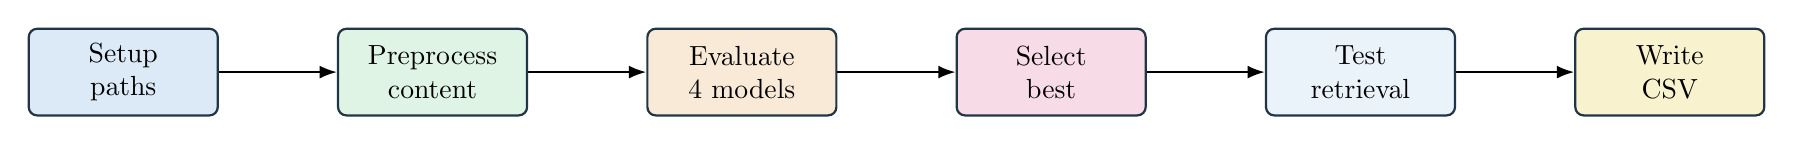
\begin{tikzpicture}[
  node distance=1.5cm,
  box/.style={draw=ink, rectangle, rounded corners=3pt, minimum width=2.4cm,
              minimum height=1.1cm, align=center, thick},
  >={Latex[length=2.2mm]}
]
\node[box, fill=softblue]   (setup)  {Setup\\paths};
\node[box, fill=softgreen,  right=of setup]  (prep)   {Preprocess\\content};
\node[box, fill=softorange, right=of prep]   (eval)   {Evaluate\\4 models};
\node[box, fill=softrose,   right=of eval]   (select) {Select\\best};
\node[box, fill=softblue!60,right=of select] (test)   {Test\\retrieval};
\node[box, fill=softgold,   right=of test]   (csv)    {Write\\CSV};

\draw[->, thick] (setup)  -- (prep);
\draw[->, thick] (prep)   -- (eval);
\draw[->, thick] (eval)   -- (select);
\draw[->, thick] (select) -- (test);
\draw[->, thick] (test)   -- (csv);
\end{tikzpicture}
}
\end{center}

\subsection{Configuration}

\begin{tabular}{>{\ttfamily}p{0.28\linewidth} p{0.60\linewidth}}
\toprule
\textbf{Parameter} & \textbf{Role} \\
\midrule
FINAL\_MODEL    & Model for submission: \texttt{bm25}, \texttt{tfidf}, \texttt{embedding}, or \texttt{hybrid}. \\
TOP\_K          & Documents per query (100). \\
OUTPUT\_PATH    & Output CSV path (\texttt{solutions\_SeaFour.csv}). \\
EMBEDDING\_MODEL & Sentence-Transformer model name (\texttt{all-MiniLM-L6-v2}). \\
EMBEDDING\_BATCH & Encoding batch size (256). \\
HYBRID\_BM25\_CANDIDATES & BM25+ candidates per query before re-ranking (500). \\
HYBRID\_ALPHA & Weight for BM25+ in score fusion, $\alpha=0.35$ by default. \\
\bottomrule
\end{tabular}

\subsection{CSV Format}

The writer reads the sample submission template, preserves column order, and
writes JSON-encoded document ID lists:

\begin{lstlisting}[language=Python]
out_row = {
    id_col: qid,
    pred_col: json.dumps(pred_map[qid]),
}
if category_col is not None:
    out_row[category_col] = row.get(category_col, '?') or '?'
\end{lstlisting}

% ═══════════════════════════════════════════════════════════════════════════════
\section{Dependencies}
% ═══════════════════════════════════════════════════════════════════════════════

\begin{tabular}{l l}
\toprule
\textbf{Package} & \textbf{Purpose} \\
\midrule
\texttt{numpy}                & Array operations and sorting \\
\texttt{pandas}               & DataFrame handling and I/O \\
\texttt{scikit-learn}         & TF-IDF vectoriser and cosine similarity \\
\texttt{rank-bm25}            & BM25+ implementation \\
\texttt{sentence-transformers} & Pre-trained dense encoders \\
\texttt{torch}                & Backend for sentence-transformers \\
\bottomrule
\end{tabular}

% ═══════════════════════════════════════════════════════════════════════════════
\appendix
\section{Mathematical Details}
% ═══════════════════════════════════════════════════════════════════════════════

\paragraph{TF-IDF.}
Weighs terms by local frequency and global rarity:
\[
\text{TF-IDF}(t,d) = \text{tf}(t,d) \cdot \log\!\left(\frac{N}{\text{df}(t)}\right)
\]

\paragraph{Cosine Similarity.}
\[
\cos(\theta) = \frac{\mathbf{q} \cdot \mathbf{d}}
  {\lVert \mathbf{q} \rVert \; \lVert \mathbf{d} \rVert}
\]

\paragraph{BM25+.}
\[
\text{BM25+}(q,d) = \sum_{t \in q} \text{IDF}(t)
\left(
  \frac{f(t,d)\,(k_1+1)}
       {f(t,d) + k_1\!\left(1 - b + b\,\frac{|d|}{\text{avgdl}}\right)}
  + \delta
\right)
\]
For comparison, standard BM25 omits the additive $\delta$ term and uses only
the saturation plus length-normalisation fraction.  BM25+ was preferred in the
notebook because once a query term is present, the extra $\delta$ keeps its
contribution positive instead of letting long-document normalisation push that
term's score too low.

\paragraph{Sentence Embedding Similarity.}
For L2-normalised vectors:
\[
\text{sim}(\mathbf{q}, \mathbf{d}) = \mathbf{q}^\top \mathbf{d}
\]

\paragraph{Hybrid Score Fusion.}
\[
\text{score}_{\text{hybrid}}(q,d)
  = \alpha \cdot \frac{\text{BM25+}(q,d) - \min}{\max - \min}
  + (1-\alpha) \cdot \text{sim}_{\text{emb}}(q,d)
\]

\paragraph{Top-K Selection.}
\[
\text{TopK}(q) = \operatorname{argsort}\!\bigl(\text{scores}(q)\bigr)[-K:][::-1]
\]

\end{document}
